\section{Linear Regression (Supervised Learning)}
Linear Regression is the most used method to analyse data. In linear regression, we  decide to only consider a linear relationship between the input and output. Most of the applications fall into two categories. \\
\textbf{Interpretation:} We want to understand if some input has an effect on the output. \textbf{Example:} Is there a
relationship between smoking cigaretts and the risk of lung cancer?\\
\textbf{Prediction:} Given some sensor data like oil pressure, temperature etc. a model could predict an engine failure.

\subsection{Machine-Learning Perspective}
We are given both the input and the labels. The ML algorithm learns the linear relationship between X and Y. The goal is to predict a $y_{i}$ for some unseen $x_{i}$. We use a model to explain the data. $y_{i}\approx f(x_{i}) + \varepsilon_{i}$ where the $\varepsilon$ is unexplained noise.

The Simplest model is the linear model with two free (unknown parameters).
$\hat{y} = ax_{i} + b$ where a=slope, b=intercept.

\subsection{Mean Squared Error (MSE)}
Is the loss we want to minimise in the ML model. $\hat{y}_{i}=a * x_{i}+b$ with the \textbf{Residual} $\varepsilon_{i}=y_{i}-\hat{y}_{i}$ Note: The sum of the squared residuals is the loss function. $E=\frac{1}{2N} \sum_{i=1}^N e_{i}^2$

\subsection{Correlations}
\begin{minipage}{0,5\linewidth}
	\textbf{Correlation is not causality!} Correlation refers to the degree to which a pair of variables are linearly related. This can be quantified with the Pearson correlation Coefficient (cov=covariant, $\sigma$=standard deviatoin).
	\[ \rho_{X,Y} = \frac{cov(X,Y)}{\sigma_{X} \sigma_{Y}}  \]  
\end{minipage}
\begin{minipage}{0,5\linewidth}
	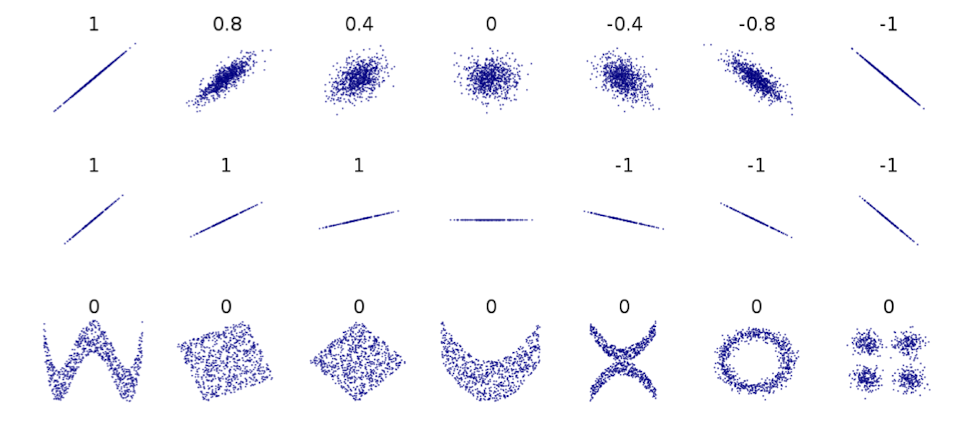
\includegraphics[width=\linewidth]{PRC}
\end{minipage}
